\documentclass[10pt,a4paper]{article}
\usepackage[utf8]{inputenc}
\usepackage[english]{babel}
\usepackage{amsmath}
\usepackage{amsfonts}
\usepackage{amssymb}
\usepackage{graphicx}
\usepackage{natbib}
\author{Fabian Schubert}
\title{Notes on Homeostasis and Plasticity in a Non-binary Recurrent Network}

\newcommand{\diff}[1]{\mathrm{d}#1}

\newcommand{\expval}[1]{\mathrm{E}[#1]}
\newcommand{\var}[1]{\mathrm{Var}[#1]}
\newcommand{\std}[1]{\mathrm{Std}[#1]}

\newcommand{\psample}{p_{\rm s}}
\newcommand{\qsample}{q_{\rm s}}
\newcommand{\ptarget}{p_{\rm t}}


\begin{document}
\maketitle





\section{Description of the Network Model}
We investigate a discrete-time, fully connected recurrent network model that includes homeostatic threshold and gain control by using the Kullback-Leibler divergence between a target distribution and neuronal output as a control measure. Standard parameters of the model are given in Table \ref{tab:parameters}. Find the details of the model in the following sections.
\begin{table}
\centering
\caption{Parameters of the network}

\begin{tabular}{l|r}
$N$ & $300$ \\
$\mathrm{E}[W]$ &  $0$\\
$\mathrm{Std}[W]$ & $1/\sqrt{N}$ \\
$\mu_b$ & $0.001$ \\
$\mu_a$ & $0.001$ \\
Initial $a$ & $1$ \\
Initial $b$ & $0$
\end{tabular}
\label{tab:parameters}
\end{table}

\subsection{Neuron Model}
At discrete times $t$, each neuron $i$ in our network is characterized by a single activity variable $y^t_i$. The next state is calculated by:
\begin{align}
y^{t+1}_i &= \sigma\left(x^t_i\right) \\
\sigma\left(x\right) &= \frac{1}{1+\exp\left(-a\left(x-b\right)\right)} \\
x^t_i &= x^t_{i,ee} + x^t_{i,eext} = \sum_j W_{ij} y^t_j  + x^t_{i,eext} \\
\end{align}
where $W_{ij}$ is a connectivity matrix whose properties are described in the following section and $x^t_{i,eext}$ is an optional external input.

\subsection{Recurrent Network Properties}
$W_{ij}$ is a fixed randomly generated matrix, whose entries were drawn from a normal distribution with mean and standard deviation given in Table \ref{tab:parameters}. Autapses were prohibited, meaning that $W_{ii} = 0$. Note that we did not impose Dale's law onto the signs of the connections.

\subsection{Gain and Threshold Control via the Kullback-Leibler Divergence}
We define by
\begin{equation}
\ptarget (y,\lambda_1,\lambda_2 ) \propto \exp\left(\lambda_1 y + \lambda_2 y^2\right)
\end{equation}
a family of Gaussian distributions as a target for the neural activity. Note that $\lambda_1$ and $\lambda_2$ are related to the target mean and variance $\mu_t,\sigma_t$ via $\lambda_1 = \mu_t/\sigma_t^2$ and $\lambda_2 = -1/\left(2 \sigma_t^2\right)$. The Kullback-Leibler divergence allows us to define a measure between the target distribution and the actual distribution---though only assessible via sampling of the output---which shall be denoted by $\psample (y)$. The K.-L. divergence is given by
\begin{align}
D_{KL}\left(p_{\rm s}||p_{\rm t}\right) &= \int \diff{y} \ \psample (y) \ln \left( \frac{\psample (y)}{\ptarget (y)} \right) \\
&= \int \diff{y} \ \qsample (x) \left[ \ln \qsample (x) - \ln\sigma '\left(x\right) - \ln \ptarget (\sigma\left(x\right)) \right]
\end{align}
where $\qsample (x)$ denotes the sampled distribution of the synaptic input or ``membrane potential". The total derivative with respect to a parameter $\theta$ of our transfer function is then given by
\begin{align}
\frac{\diff{D}}{\diff{\theta}} &= -\int \diff{x} \ \qsample (x) \sigma'^{-1} \left(x\right) \frac{\partial \sigma'}{\partial \theta} \left( x\right) - \int \diff{x} \ \qsample (x) \frac{\ptarget'(x)}{ \ptarget(x)} \frac{\partial \sigma}{\partial \theta} (x) \\
&\equiv \int \diff{x} \ \qsample (x) \frac{\partial d(x)}{\partial \theta} \; .
\end{align}

We then used this expression to derive on-line local adaptation rules for the gain $a$ and threshold $b$ by steepest decent:
\begin{align}
a^{t+1}_i &= a^t_i + \Delta a^t_i \\
b^{t+1}_i &= b^t_i + \Delta b^t_i \\
\Delta a^t_i &= - \epsilon_a \frac{\partial d(x^t_i)}{\partial a_i} = \epsilon_a \frac{1}{a^t_i}\left[ 1 - \ln \left( \frac{1}{y^t_i} - 1 \right) \Theta^t_i \right] \\
\Delta b^t_i &= - \epsilon_b \frac{\partial d(x^t_i)}{\partial b_i} = \epsilon_b \left(-a^t_i\right) \Theta^t_i \\
\Theta^t_i &\equiv 1-2y^t_i + y^t_i (1-2y^t_i)[\lambda_1 + 2\lambda_2 y^t_i] \label{eq:theta}
\end{align}

Note that, aside from a scaling factor, gain and threshold dynamics can be expressed solely in terms of output activity and target parameters. This allows us to find dynamical fixed points of $a$ and $b$ in terms of the output activity.

\begin{figure}
\centering
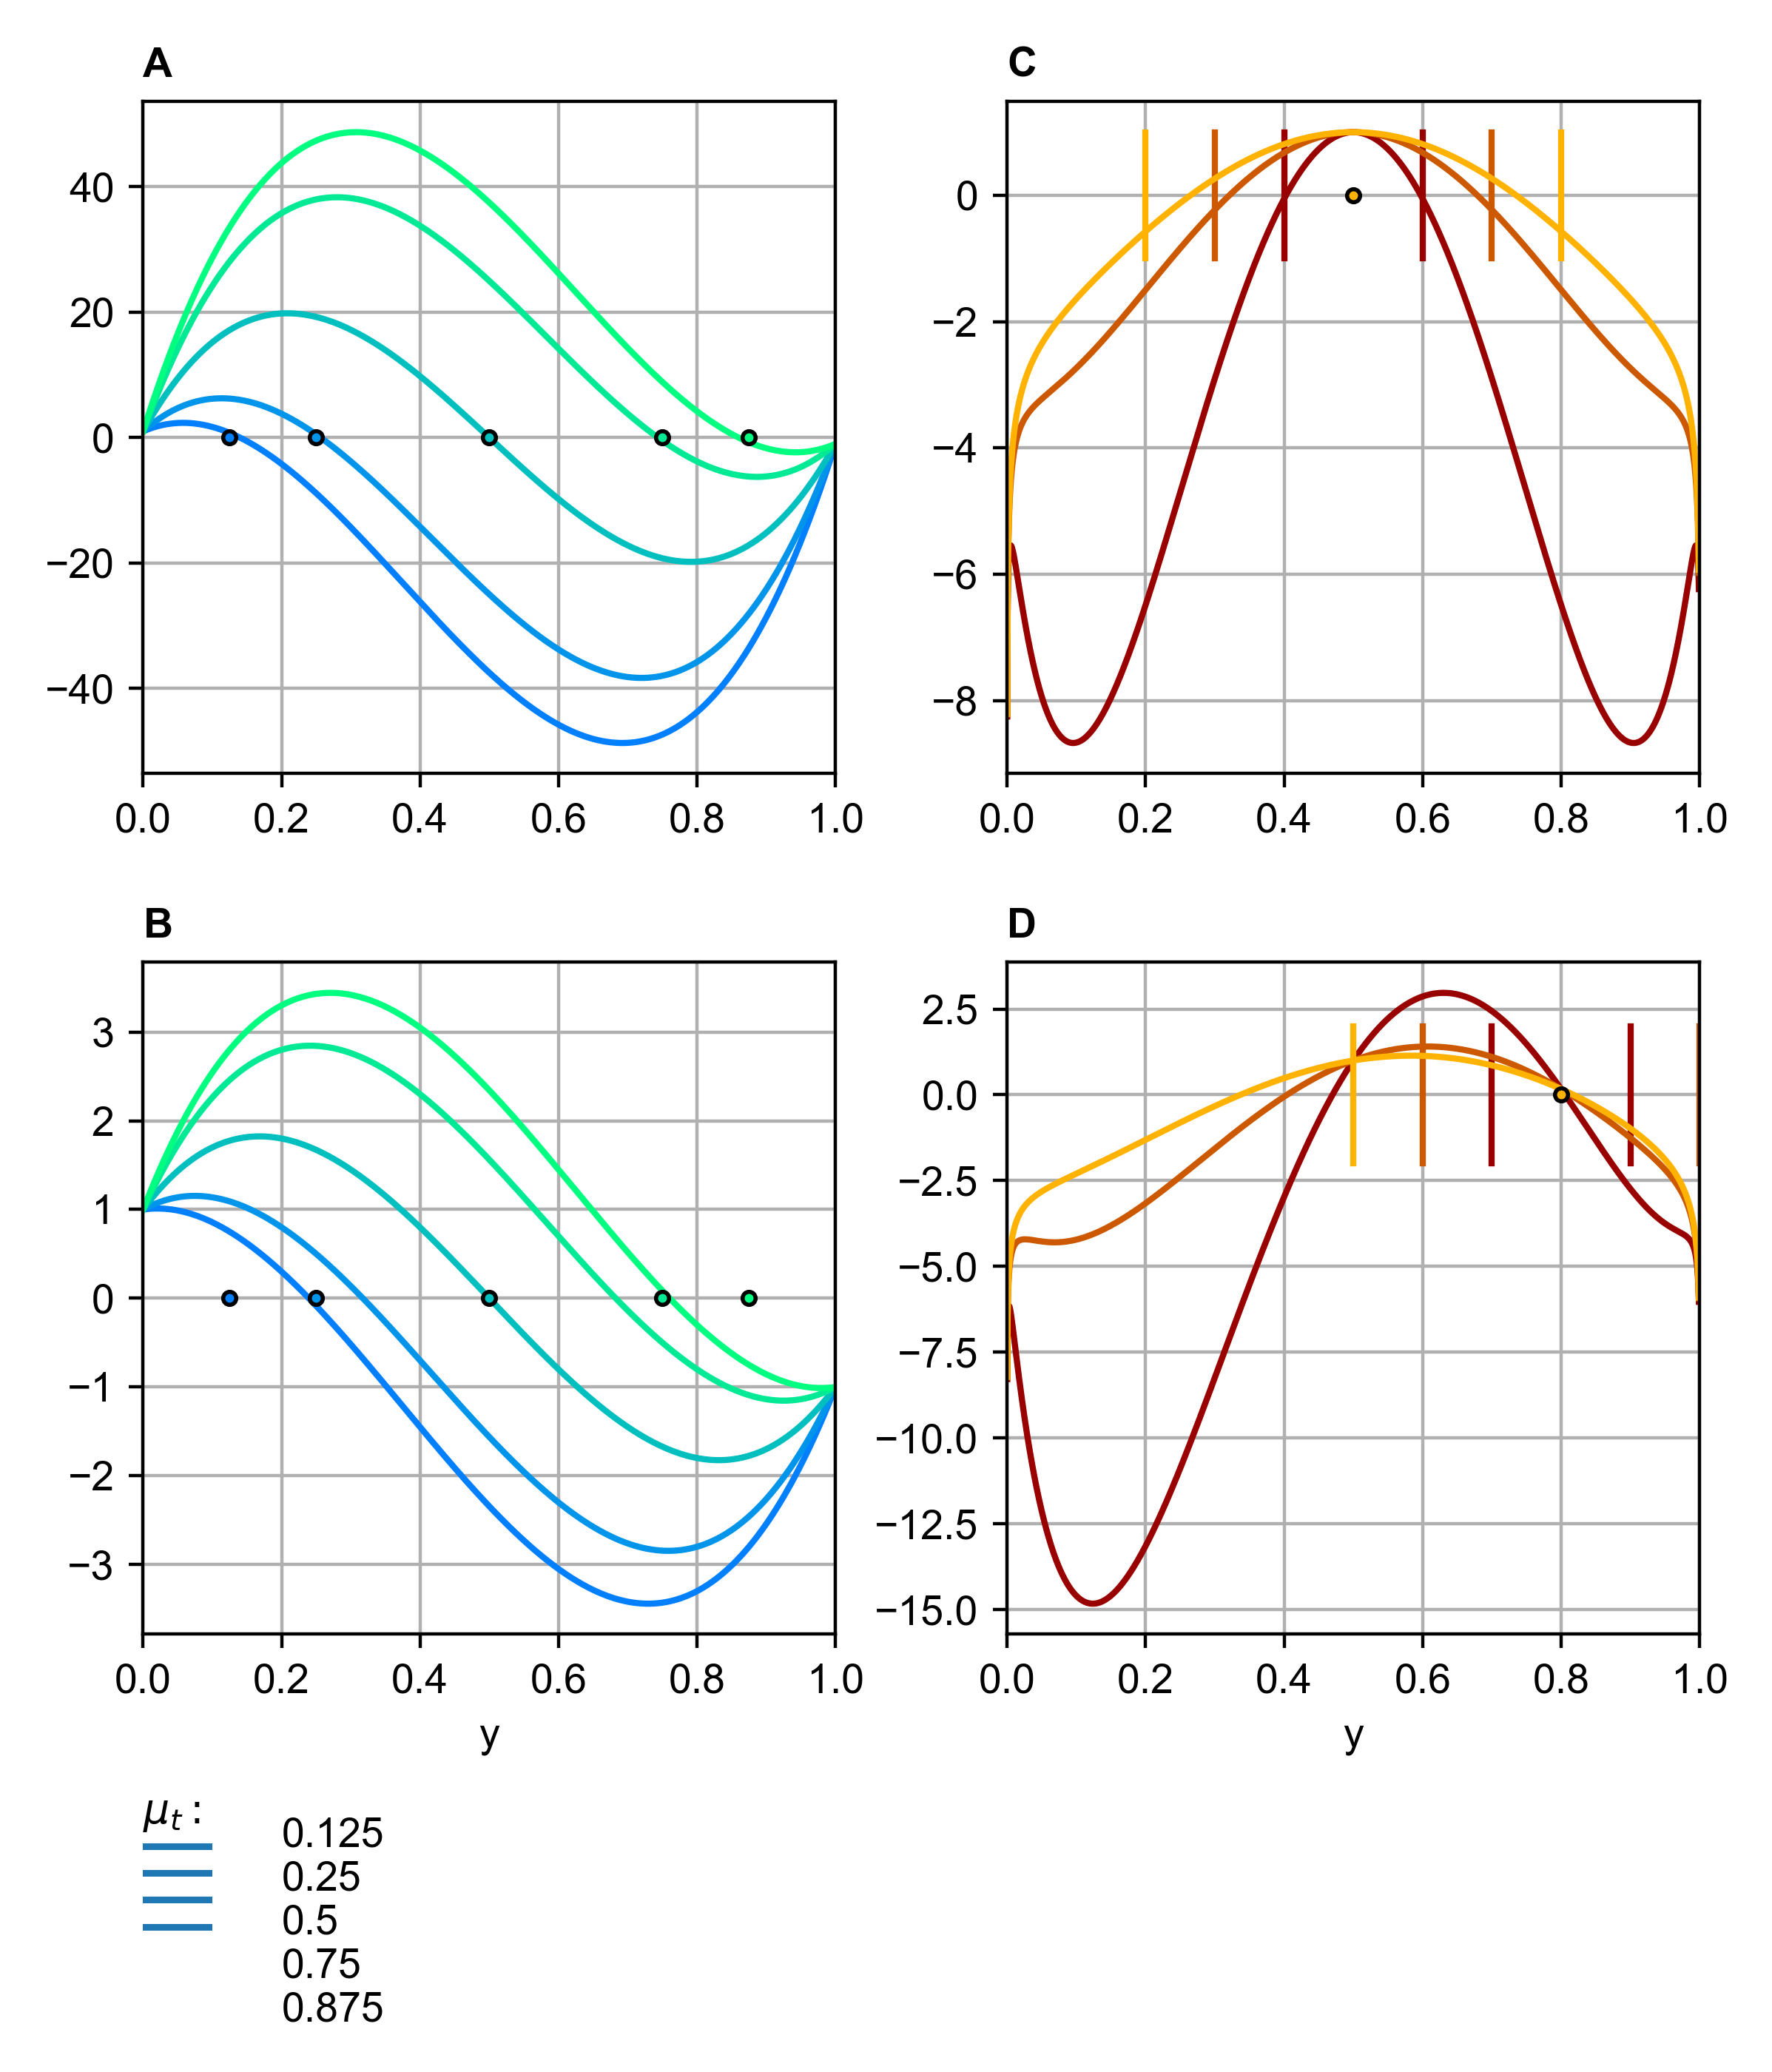
\includegraphics[width=\textwidth]{./figures/gain_thresh_dyn.png}
\caption{\textbf{A},\textbf{B}: $\Theta$ as a function of $y$ as given in \eqref{eq:theta}. }
\end{figure}



\bibliographystyle{unsrt}
\bibliography{/home/fschubert/work/lit_base.bib}

\end{document}